% ===================== MP-Bench =====================
\subsection{MP-Bench}\label{ds:mp_bench}
\badgerow{\naturalbadge\ \okbadge\ \lbl{step set + category, 3 annotators}\ \lbl{MAS}\ \lbl{GAIA / AssistantBench}\ \lbl{re-annotates Who\&When + MAST logs}}

\begin{identity}
Paper & \emph{Rethinking Failure Attribution in Multi-Agent Systems: A Multi-Perspective Benchmark and Evaluation} --- In, Tanjim, Subramanian, Kim, Bhattacharya, Kim, Park, Sarkhel, Park (KAIST / Adobe Research), arXiv:2603.25001 (2026; ICML 2026 FAGEN Workshop / KDD 2026 AgenticSE Workshop) \cite{mpbench2026}\\
Links & \href{https://github.com/adobe-research/multi-agent-eval-bench}{GitHub \code{adobe-research/multi-agent-eval-bench}} (annotations) \textperiodcentered\ \href{https://github.com/yeonjun-in/MP-Bench}{GitHub \code{yeonjun-in/MP-Bench}} (evaluation pipeline, leaderboard) \textperiodcentered\ \href{https://yeonjun-in.github.io/MP-Bench/}{leaderboard page}; the HF mirror \code{Yeonjun/MP-Bench} holds only README + LICENSE\\
License & Adobe Research License v1.2 (non-commercial research/teaching only; derivatives must stay non-commercial); the pointed-to logs keep their own terms (Who\&When: none stated; MAST repo: MIT)\\
Status & downloaded in full, ungated; 2.7 MB annotations (4.8 MB on disk) + 0.2 MB eval code + 14.1 MB fetched source logs (15.5 MB on disk). The release ships \emph{annotation pointers only}: all 289 source logs were fetched from the Who\&When and MAST GitHub repos with our own script; \code{data/attribution/mp\_bench/}\\
\end{identity}

\paragraph{Description} MP-Bench argues that failure attribution is \emph{non-deterministic}: a failed MAS log usually admits several plausible root causes, so a benchmark should store a \emph{set} of expert perspectives rather than one gold (agent, step). It re-annotates 289 existing, naturally occurring MAS logs (no injection; 121 nominal configurations---1 manual + 120 automatic tasks spanning 118 distinct \code{system\_prompt}s and 116 agent sets); while framed as failed runs (all 177 Who\&When logs failed), 26 of the 112 MAST logs (24 L2, 2 L3) exact-match \code{expected\_answer.txt}, 12 of which carry empty annotations from all three annotators (leaving 157 scored manual logs on the leaderboard; the other 14 still receive step-level flags):
\begin{itemize}
\item \textbf{manual} (169 logs, hand-crafted MAS): 57 Who\&When Hand-Crafted Magentic-One logs plus 112 Magentic-One GAIA-validation console logs (86 level-2, 26 level-3) from the MAST failure-taxonomy corpus.
\item \textbf{automatic} (120 logs, algorithm-generated MAS): the Who\&When Algorithm-Generated CaptainAgent logs.
\end{itemize}
\textbf{Annotation}: three experts recruited on Upwork after a two-stage screening labelled \emph{every} log independently, with no guiding perspective: per step a binary failure-inducing flag, a free-text \code{fail\_reason}, a counterfactual \code{ideal\_action} and a \code{fail\_category} from 9 classes (8 ending in ``Error'': Planning, Verification, Reasoning, Contextual Understanding, Tool Usage, Tool/Agent Invocation, Resource Access, System Error, plus Reasoning--Action Mismatch---not formally defined in the paper; 2 of 4,418 flags leave \code{fail\_category} empty). $\approx$31 min per manual and 14 min per automatic log, $\approx$346 expert-hours. \textbf{Agreement} is low by design: of all flagged steps 16.2\% are flagged by all three annotators, 27.8\% by two, 56.1\% by one (paper); pairwise disagreement reaches $\approx$60\%. Each step gets a \emph{consensus rate} (fraction of annotators flagging it), and GPT-5.1 consolidates the annotators' reasons and ideal actions per step.

\paragraph{Metrics and baselines} The attributor outputs a \emph{ranked list} of failure steps with reasons (three seeds, consolidated). \emph{Attribution}: nDCG@5 (and nDCG@all) of that ranking against the consensus ranking; \emph{reasoning}: GPT-5.1 judge scores (1--10) for fail reason, ideal action and overall agreement with the consolidated annotator rationale. All-at-Once with taxonomy, nDCG@5 (exponential gain) / judge average (paper):

\begin{center}\small
\begin{tabular}{@{}lcc@{}}\toprule
Model & Hand-crafted & Automatic\\\midrule
Random & 0.128 / -- & 0.315 / --\\
GPT-4.1 & 0.431 / 7.63 & 0.676 / 7.78\\
GPT-5.1 & 0.375 / 7.62 & 0.784 / \textbf{8.25}\\
o3-mini & 0.437 / 7.48 & 0.394 / 7.37\\
Claude Sonnet 4.5 & \textbf{0.440} / \textbf{7.95} & \textbf{0.789} / 8.23\\
Qwen3-8B & 0.294 / 6.11 & 0.668 / 6.54\\
GPT-oss-120B & 0.425 / 7.51 & 0.703 / 7.92\\\bottomrule
\end{tabular}
\end{center}
Under this multi-perspective view LLMs are far from random---the opposite conclusion to Who\&When's single-label step accuracy. The public leaderboard (\code{leaderboard.json}) uses nDCG@5 only (157 manual + 120 automatic logs scored, excluding the 12 all-empty manual logs) and differs slightly from the paper table, ranking GPT-oss-120B (0.449) and GPT-4.1 (0.445) above Claude Sonnet 4.5 (0.432; o3-mini omitted).

\paragraph{Schema} \code{MP-Bench/<annotator 1--3>/<manual|automatic>/<n>.json} (867 files = 3$\times$289): \code{log\_source} (GitHub URL of the Who\&When JSON or the MAST \code{console\_log.txt}) and \code{annotation}, a possibly empty list of \{\code{step}, \code{fail\_annotation} (``1''), \code{fail\_category}, \code{fail\_reason}, \code{ideal\_action}\}; \code{step} is a 0-based index (stored as a string) into the step list built by the official \code{build\_annotated\_from\_log\_source.py}: Who\&When \code{history} entries, or MAST console turns split on \code{---------- <Agent> ----------} delimiters (question from \code{prompt.txt}, answer from \code{expected\_answer.txt}). The normalised form is \{\code{question}, \code{ground\_truth}, \code{is\_correct}, \code{system\_prompt}, \code{history}:[\{\code{content}, \code{role}, \code{step}, + the four label fields\}]\}; in practice \code{is\_correct} (always \code{False}) and \code{system\_prompt} are populated only for the 120 automatic logs (\code{None} / \code{\{\}} for all 169 manual logs, since W\&W HC uses \code{is\_corrected} and MAST omits both), 91/289 logs contain literal \code{<image>} placeholders with no image files, and token counts, timestamps, and structured tool-call payloads are absent. Our copy keeps the fetched logs under \code{data/attribution/mp\_bench/sources/<sha1(url)[:16]>/} with an \code{index.json} map.

\paragraph{Statistics} computed from the full downloaded corpus of all 289 logs (169 manual + 120 automatic; 867 annotation files, 4,418 flags total).\par\nobreak\vspace{1pt}
\noindent\begin{minipage}[t]{0.54\linewidth}\vspace{0pt}\small
{\footnotesize\setlength{\tabcolsep}{3.5pt}\fitbox{\begin{tabular}{@{}lrrr@{}}\toprule
 & All & manual & automatic\\\midrule
logs analysed (26 MAST exact-match) & 289 & 169 & 120\\
W\&W HC / MAST L2+L3 / W\&W AG & 57 / 86+26 / 120 & 57 / 86+26 / -- & -- / -- / 120\\
steps: mean / median & 23.9 / 10 & 34.7 / 29 & 8.7 / 10\\
steps: min -- max & 5 -- 130 & 5 -- 130 & 5 -- 10\\
distinct MAS agents: mean (max)$^*$ & 3.1 (5) & 2.8 (5) & 3.6 (4)\\
flags per annotator-log: mean / max & 5.1 / 59 & 6.5 / 59 & 3.1 / 10\\
flagged steps per log (union): mean / max & 9.5 / 78 & 12.6 / 78 & 5.3 / 10\\
steps with 1 / 2 / 3 votes & 1547 / 765 / 447 & 1239 / 579 / 305 & 308 / 186 / 142\\
earliest majority, rel.\ pos.\ (mean / med.)$^\dagger$ & 0.40 / 0.33 & 0.44 / 0.35 & 0.36 / 0.30\\
characters / log: mean & 34.5\,k & 50.7\,k & 11.6\,k\\\bottomrule
\end{tabular}}}

\smallskip Consensus across all 289 logs: 56.1\% / 27.7\% / 16.2\% of flagged steps carry 1 / 2 / 3 votes (matching the paper's 56.1 / 27.8 / 16.2). $^*$Normalised MAS roles excluding \code{user}/\code{human} prompts (including them: 3.7 (6) all, 3.8 (6) manual). $^\dagger$1-based $(s{+}1)/n$ over the 264/289 logs with a $\ge$2-vote step (145 manual, 119 automatic; 25 have none). Agent share of per-annotator flags, manual ($n{=}3{,}312$): combined orchestrators 58.1\% (\code{MagenticOneOrchestrator} 31.5\% + \code{Orchestrator} 26.6\%), \code{WebSurfer} 32.2\%, \code{FileSurfer} 3.8\%, \code{Assistant} 3.8\%; automatic ($n{=}1{,}106$): \code{Verification\_Expert} 17.1\%, \code{Computer\_terminal} 9.2\%, \code{Validation\_Expert} 6.1\%, \code{DataVerification\_Expert} 4.5\%, the rest spread over many \code{*\_Expert} roles (by unique flagged steps, $n{=}636$, \code{Computer\_terminal} 15.3\% edges out \code{Verification\_Expert} 14.9\%).
\end{minipage}\hfill
\begin{minipage}[t]{0.44\linewidth}\vspace{0pt}
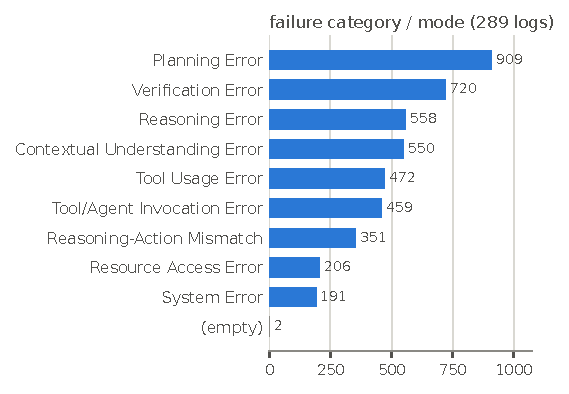
\includegraphics[width=\linewidth]{3_core/mp_bench/figures/cat.pdf}
\end{minipage}

\paragraph{Example trajectory} \code{manual/18.json} (MAST Magentic-One GAIA level-2 log; 9 steps, 2 MAS agents plus \code{user}, 13.7\,k characters). The first Bing search already shows ``beta-geometric'' in a snippet; the WebSurfer's click on a paper silently fails, it then summarises ``Markov models'' and the orchestrator answers \emph{Markov Model} (ground truth \emph{beta geometric}). Five steps are flagged in total: 5, 7 and 8 by all three annotators, 3 only by annotator 3, 6 only by annotator 2---the renderer marks all five; the annotation box lists the per-annotator (step, annotator, category) labels with their reasons (truncated) and the per-step votes, and its ``faulty agent'' row names only the agent of the first flagged step (steps 6 and 8 blame the orchestrator).
% auto-generated by scripts/render_traj.py -- do not edit
\trajtask{manual/\allowbreak{}18.json}{What two-word type of model did Manash Pratim Kashyap's and PS Fader's studies in customer retention studies published during 2018-2019 have in common (no punctuation)?\allowbreak{}}
\begin{trajstep}{0}{user}{agA}
What two-word type of model did Manash Pratim Kashyap's and PS Fader's studies in customer retention studies published during 2018-2019 have in common (no punctuation)?\allowbreak{}
\end{trajstep}
\begin{trajstep}{1}{MagenticOneOrchestrator}{agB}
We are working to address the following user request:\allowbreak{}\par What two-word type of model did Manash Pratim Kashyap's and PS Fader's studies in customer retention studies published during 2018-2019 have in common (no punctuation)?\allowbreak{}\par To answer this request we have assembled the following team:\allowbreak{}\par Assistant:\allowbreak{} A helpful and general-purpose AI assistant that has strong language skills,\allowbreak{} Python skills,\allowbreak{} and Linux command line skills.\newline ComputerTerminal:\allowbreak{} A computer terminal that performs no other action than running Python scripts (provided to it quoted in ```python code blocks),\allowbreak{} or sh shell scripts (provided to it quoted in ```sh code blocks).\newline FileSurfer:\allowbreak{} An\newline [...] (2,\allowbreak{}197 chars omitted) [...]\newline tion studies.\par - **Assistant Task**:\allowbreak{} Conclude by presenting the likely common two-word model based on the information obtained.\par The focus will be on employing WebSurfer to locate and extract pertinent information about the studies and the models used.
\end{trajstep}
\begin{trajstep}{2}{MagenticOneOrchestrator}{agB}
Please conduct a search for academic publications or articles by Manash Pratim Kashyap and PS Fader on customer retention from 2018-2019. Focus on identifying the type of models used in these studies and look for a two-word model that is common to both.
\end{trajstep}
\begin{faultystep}{3}{WebSurfer}{agC}
I typed 'Manash Pratim Kashyap PS Fader customer retention model 2018-2019' into the browser search bar.\par The web browser is open to the page [Manash Pratim Kashyap PS Fader customer retention model 2018-2019 - Cerca](https:\allowbreak{}/\allowbreak{}/\allowbreak{}www.bing.com/\allowbreak{}search?\allowbreak{}q=\allowbreak{}Manash+Pratim+Kashyap+PS+Fader+customer+retention+model+2018-2019\&FORM=\allowbreak{}QBLH).\newline The viewport shows 39\% of the webpage,\allowbreak{} and is positioned at the top of the page\newline The following text is visible in the viewport:\allowbreak{}\par Microsoft e i suoi fornitori di terze parti utilizzano cookie e tecnologie simili per fornire,\allowbreak{} gestire e migliorare i servizi e gli annunci offerti. Se sei d'accordo,\allowbreak{} useremo questi dati per la\newline [...] (4,\allowbreak{}140 chars omitted) [...]\newline "fb:\allowbreak{}app\_id":\allowbreak{} "3732605936979161",\allowbreak{}\newline "og:\allowbreak{}image":\allowbreak{} "http:\allowbreak{}/\allowbreak{}/\allowbreak{}www.bing.com/\allowbreak{}sa/\allowbreak{}simg/\allowbreak{}facebook\_sharing\_5.png",\allowbreak{}\newline "og:\allowbreak{}type":\allowbreak{} "website",\allowbreak{}\newline "og:\allowbreak{}image:\allowbreak{}width":\allowbreak{} "600",\allowbreak{}\newline "og:\allowbreak{}image:\allowbreak{}height":\allowbreak{} "315"\newline \}\newline \}\par Here is a screenshot of the page.\newline <image>
\end{faultystep}
\begin{trajstep}{4}{MagenticOneOrchestrator}{agB}
Please check the search results for any documents or mentions that specify the model type used by both Manash Pratim Kashyap and PS Fader in their customer retention studies from 2018-2019.
\end{trajstep}
\begin{faultystep}{5}{WebSurfer}{agC}
I clicked 'A Simple Model for Analyzing the Customer Retention Comparing Rural and Urban Store'.\par The web browser is open to the page [Manash Pratim Kashyap PS Fader customer retention model 2018-2019 - Cerca](https:\allowbreak{}/\allowbreak{}/\allowbreak{}www.bing.com/\allowbreak{}search?\allowbreak{}q=\allowbreak{}Manash+Pratim+Kashyap+PS+Fader+customer+retention+model+2018-2019\&FORM=\allowbreak{}QBLH).\newline The viewport shows 39\% of the webpage,\allowbreak{} and is positioned at the top of the page\newline The following text is visible in the viewport:\allowbreak{}\par Microsoft e i suoi fornitori di terze parti utilizzano cookie e tecnologie simili per fornire,\allowbreak{} gestire e migliorare i servizi e gli annunci offerti. Se sei d'accordo,\allowbreak{} useremo questi dati per la personal\newline [...] (3,\allowbreak{}091 chars omitted) [...]\newline E CUSTOMER RETENTION ...31 mar 2019 \textperiodcentered{} The aim of this study is to explore relationships among five factors:\allowbreak{} customer relationship management,\allowbreak{} customer satisfaction,\allowbreak{} customer loyalty,\allowbreak{} customer profitability,\allowbreak{} and ...\newline Here is a screenshot of the page.\newline <image>
\end{faultystep}
\begin{faultystep}{6}{MagenticOneOrchestrator}{agB}
Please extract more detailed information from the identified webpage,\allowbreak{} focusing on the specific type of model mentioned in the studies,\allowbreak{} and verify if it matches a two-word model type used by both authors.
\end{faultystep}
\begin{faultystep}{7}{WebSurfer}{agC}
The studies by Manash Pratim Kashyap and others,\allowbreak{} including PS Fader,\allowbreak{} during 2018-2019,\allowbreak{} primarily mention customer retention models that include the use of Reinartz and Kumar's model from 2000,\allowbreak{} as well as a modified version by Fader,\allowbreak{} Hardie,\allowbreak{} and Lee in 2005. These models focus on assessing customer retention by evaluating customer switching behaviors and often employ migration or Markov models to estimate the probabilities of customers transitioning between states. The models emphasize analyzing customer relationship dynamics between rural and urban stores,\allowbreak{} helping in the prediction of future purchase patterns by leveraging structural characteristics and retention estimates.
\end{faultystep}
\begin{faultystep}{8}{MagenticOneOrchestrator}{agB}
FINAL ANSWER:\allowbreak{} Markov Model\newline SCENARIO.PY COMPLETE !\#!\#\newline SCENARIO.PY RUNTIME:\allowbreak{} 494 !\#!\#\newline RUN.SH COMPLETE !\#!\#
\end{faultystep}
\trajannotation{WebSurfer}{3,\allowbreak{} 5,\allowbreak{} 6,\allowbreak{} 7,\allowbreak{} 8}{["Contextual Understanding Error",\allowbreak{} "Reasoning Error",\allowbreak{} "Reasoning-Action Mismatch",\allowbreak{} "Tool Usage Error",\allowbreak{} "Tool/\allowbreak{}Agent Invocation Error",\allowbreak{} "Verification Error"]}{[step 3,\allowbreak{} annotator 3,\allowbreak{} Tool/\allowbreak{}Agent Invocation Error] Found search results containing 'beta-geometric (BG) distribution' reference but failed to highlight or extract this key information for the task;\allowbreak{} [step 5,\allowbreak{} annotator 1,\allowbreak{} Tool Usage Error] WebSurfer attempted to click on the Academia.edu link 'A Simple Model for Analyzing the Customer Retention Comparing Rural and Urban Store' but the navigation failed. The browser remained on the Bing search results page instead of navigating to the actual article. This prevented WebSurfer from accessing the detailed content of Kashyap's paper which would have provided more specific model information.;\allowbreak{} [step 5,\allowbreak{} annotator 2,\allowbreak{} Reasoning-Action Mismatch] The agent says it clicked a paper,\allowbreak{} but the page content did not change and no paper was opened.;\allowbreak{} [step 5,\allowbreak{} annotator 3,\allowbreak{} Tool/\allowbreak{}Agent Invocation Error] Failed to navigate to the academic paper,\allowbreak{} clicking did not successfully access the detailed content needed for analysis;\allowbreak{} [step 6,\allowbreak{} annotator 2,\allowbreak{} Verification Error] The Orchestrator did not verify whether the WebSurfer had actually opened a p\newline [...] (1,\allowbreak{}003 chars omitted) [...]\newline swer 'beta geometric' was clearly visible in the search results;\allowbreak{} [step 8,\allowbreak{} annotator 2,\allowbreak{} Verification Error] The Orchestrator finalized the answer without verifying whether the information from earlier steps was correct or supported by real sources.;\allowbreak{} [step 8,\allowbreak{} annotator 3,\allowbreak{} Reasoning Error] Concluded with 'Markov Model' instead of 'beta geometric' despite evidence in search results pointing to beta-geometric distribution}{beta geometric}{FINAL ANSWER:\allowbreak{} Markov Model\newline SCENARIO.PY COMPLETE !\#!\#\newline SCENARIO.PY RUNTIME:\allowbreak{} 494 !\#!\#\newline RUN.SH COMPLETE !\#!\#}{\textbf{per\_annotator}: \{"1":\allowbreak{} [\{"step":\allowbreak{} "5",\allowbreak{} "fail\_annotation":\allowbreak{} "1",\allowbreak{} "fail\_category":\allowbreak{} "Tool Usage Error",\allowbreak{} "fail\_reason":\allowbreak{} "WebSurfer attempted to click on the Academia.edu link 'A Simple Model for Analyzing the Customer Retention Comparing Rural and Urban Store' but the navigation failed. The browser remained on the Bing search results page instead of navigating to the actual articl\newline [...] (4,\allowbreak{}490 chars omitted) [...]\newline he search results more carefully and identified 'beta geometric' as the common model type based on the Fader and Hardie (2007) reference"\}]\}; \textbf{votes\_per\_step}: \{"5":\allowbreak{} ["1",\allowbreak{} "2",\allowbreak{} "3"],\allowbreak{} "7":\allowbreak{} ["1",\allowbreak{} "2",\allowbreak{} "3"],\allowbreak{} "8":\allowbreak{} ["1",\allowbreak{} "2",\allowbreak{} "3"],\allowbreak{} "6":\allowbreak{} ["2"],\allowbreak{} "3":\allowbreak{} ["3"]\}; \textbf{earliest\_majority\_step}: 5; \textbf{source\_kind}: MAST/\allowbreak{}MagenticOne\_GAIA L2; \textbf{log\_source}: https:\allowbreak{}/\allowbreak{}/\allowbreak{}github.com/\allowbreak{}multi-agent-systems-failure-taxonomy/\allowbreak{}MAST/\allowbreak{}tree/\allowbreak{}main/\allowbreak{}traces/\allowbreak{}MagenticOne\_GAIA/\allowbreak{}gaia\_validation\_level\_2\_\_MagenticOne/\allowbreak{}0ff53813-3367-4f43-bcbd-3fd725c1bf4b/\allowbreak{}0/\allowbreak{}console\_log.txt; \textbf{is\_correct}: None; \textbf{step\_indexing}: 0-based index into reconstructed history (Who\&When JSON history /\allowbreak{} MAST console-log turns)}


\paragraph{Notes} (i) No single gold label: each log has three independent annotation sets, annotators flag several steps each (mean 5.1 per annotator-log, union mean 9.5, max 78), and the task is ranking/set prediction, not ``find the decisive step''. The ``earliest majority-flagged step'' position (0.40, 1-based over the 264 logs with $\ge$2-vote steps) is our derived quantity for comparability, not an official label. (ii) Categories are per flag and per annotator---the same step often receives different categories (step 5 of the example: Tool Usage / Reasoning--Action Mismatch / Tool/Agent Invocation); \code{ideal\_action} is unique to this dataset. (iii) Pointer-only release: trajectories must be fetched from the Who\&When and MAST repos, and step indices depend on the official parser (we re-implemented it rather than executing it); MAST logs name the orchestrator \code{MagenticOneOrchestrator} and start with the raw \code{user} prompt, Who\&When HC logs start with \code{human} and use \code{Orchestrator (thought)} / \code{Orchestrator (-> X)}. (iv) Counts differ across sources (README 289 / 121 MAS; eval README 169 + 126; \code{run.sh} loops 1--58 manual / 1--126 automatic; released files 169 + 120; leaderboard 157 + 120, excluding 12 all-empty MAST logs)---treat 289 (169 / 120) as canonical. (v) Overlap: 177 of the 289 logs are Who\&When logs re-annotated, a direct test of label reliability (the three annotators frequently disagree with each other and with Who\&When's single decisive step); the other 112 are output-only Magentic-One console logs from MAST. Automatic (5--10 step) logs are much easier (nDCG $\approx$0.7--0.8) than hand-crafted ones ($\approx$0.4). (vi) Non-commercial licence; the consolidation and judge steps of the evaluation need paid API models, and the released eval repo omits \code{taxonomy.txt} required by \code{evaluate\_all\_at\_once\_taxonomy}.
